To evaluate the performance of our system we perform experiments that draw comparisons in terms of quantitative pose estimation and qualitative reconstruction quality and efficacy.
Firstly, pose estimation is evaluated against a well established dense SLAM evaluation benchmark \cite{sturm12iros}, with the primary difference being that with traditional dense SLAM 
systems \cite{Prisacariu2014,Niessner2013,Newcombe2011}, for which the benchmark is often used, the entire visible scene is used for pose estimation, whereas in our system only the object 
surface is tracked. Qualitative comparisons are also drawn between the reconstructions of our system versus those of the system described in \cite{Ren2013}.

We evaluate our system on a set of objects of different sizes, some sequences with the object moving, others with the camera moving in the case of qualitative evaluation. 

\subsection{Pose Estimation Quality}
In this section we present quantitative results of our systems ability to maintain tracking robustness when tracking only an object and not the scene. In addition, the outputted trajectories 
of our system demonstrate less tracking drift and a robustness to loop closure events. We evaluate on <N> sequences of objects where the motion is of the camera, as such the evaluation is of 
camera pose estimation when tracking an object. At this point it should be highlighted that our system is at a disadvantage when compared to dense SLAM systems that utilise the entire scene 
geometry for pose optimisation.

In the following experiments, tracking is performed using only geometry cues from the rendered object models and the instantaneous depth frame.\\

Tracking is evaluated w.r.t. ATE(Absolute Trajectory Error) as outlined in \cite{sturm12iros} and is summarised in Table \ref{ateTable}
\begin{table}[!t]
	{\small
		\begin{center}
			\begin{tabular}{l@{\hskip 1cm} c c}
				\emph{Sequence Name} & \emph{ATE}\\
				\midrule
				\textsf{freiburg3\_cabinet} & 0.077903\\
				\textsf{freiburg3\_teddy} & 0.030596\\
			\end{tabular}
		\end{center}
	}
	\caption{The absolute trajectory error (ATE) results (in metres, lower is better) achieved by our approach in comparison to the baseline.}
	\label{ateTable}
\end{table}

\begin{figure}[!t]
	\centering
	\begin{tabular}{cccc}
		\bmvaHangBox{\fbox{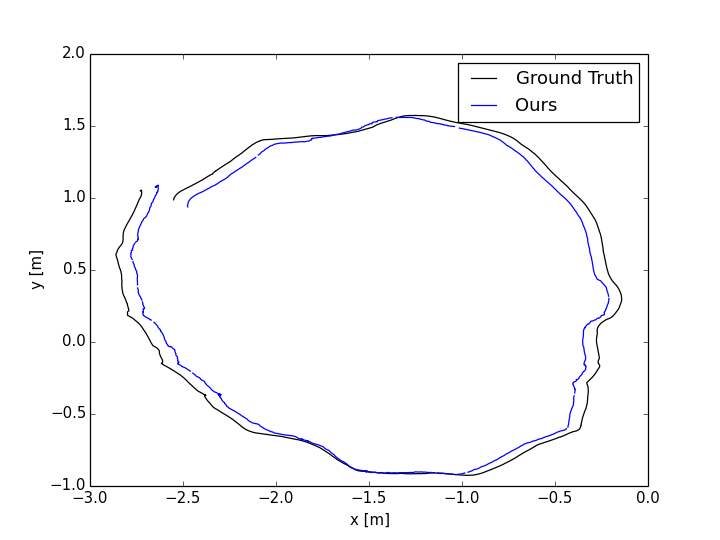
\includegraphics[scale=0.15]{results/rgbd_dataset_freiburg3_cabinet.png}}}&
		\bmvaHangBox{\fbox{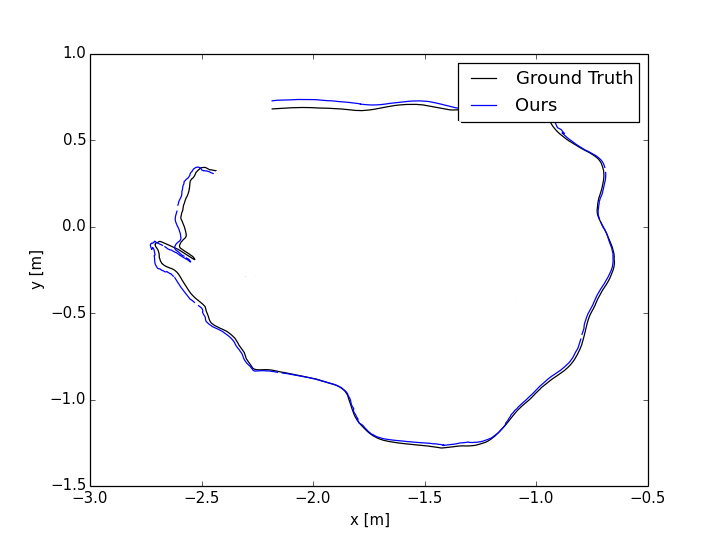
\includegraphics[scale=0.15]{results/rgbd_dataset_freiburg3_teddy.png}}}&\\
		(a)&(b)
	\end{tabular}
	\caption{
		\textbf{(a)} Trajectory of the camera for the \textit{freiburg3\_cabinet} sequence versus ground truth.
		\textbf{(b)} Trajectory of the camera for the \textit{freiburg3\_teddy} sequence versus ground truth.
	}
\label{fig:tumTrajectories}
\end{figure}

As can be seen by the presented results, our system is able to robustly estimate poses with close to ground truth quality when using only the objects geometry. In the \textit{freiburg3\_cabinet} sequence, 
there is little useful geometry available as the object is mostly planar. It can be seen that there is a small deficit in tracking quality due to this factor, however our system is still able to maintain an 
overall robust trajectory. 
In the \textit{freiburg3\_teddy} sequence we achieve a very close to ground truth trajectory, with an improvement over \textit{freiburg3\_cabinet} due to the increase in geometrical features, such as the 
curves of the teddy's body and head.

\subsection{Qualitative Reconstruction Quality}
In this section we present a qualitative evaluation of our method vs the work of Ren et al \cite{Ren2013} in the reconstruction of closed object models. We use a variety of sequences and demonstrate 
efficacy over \cite{Ren2013} in this regard. Each sequence is run through our system and that of \cite{Ren2013} with snapshots of the reconstruction in the case of our system and level set evolutions 
in the case of \cite{Ren2013}, at quarterly intervals of the systems run time through the sequence.

\begin{figure}[!t]
	\centering
	\begin{tabular}{cccc}
		\bmvaHangBox{\fbox{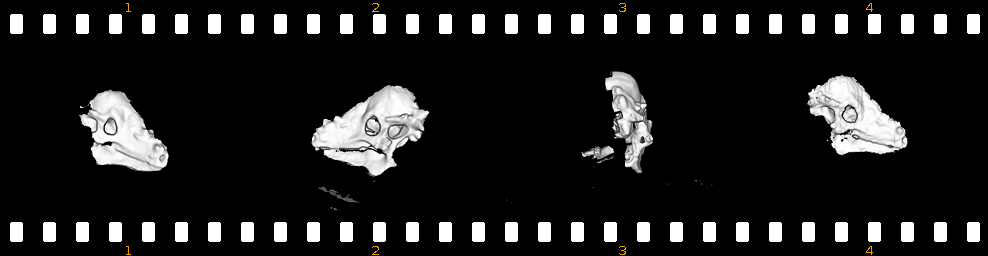
\includegraphics[scale=0.2]{filmstrips/dino.png}}}&\\
		(a)\\
		\bmvaHangBox{\fbox{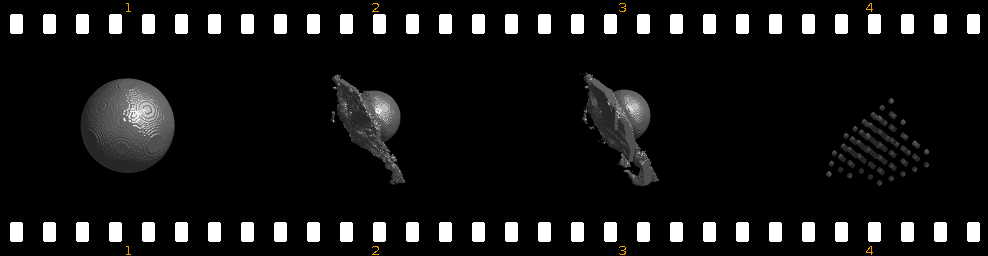
\includegraphics[scale=0.2]{filmstrips/dino_s3d_large.png}}}&\\
		(b)
	\end{tabular}
	\caption{
		\textbf{(a)} Quarterly interval snapshots of the Dinosaur Head reconstruction using our method.
		\textbf{(b)} Quarterly interval snapshots of the Dinosaur Head level set evolution using the method of Ren et al.
	}
	\label{fig:dinoComparison}
\end{figure}

As can be seen in Figure \ref{fig:dinoComparison} our method is able to successfully reconstruct the Dinosaur Head whereas the method of Ren et al fails to converge towards a feasible shape. In addition, 
Figure \ref{fig:top_shots} demonstrates that our system is able to generate closed models for a variety of sequences with the presence of loop closure. The failure of the method of Ren et al is 
also apparent for other sequences used in this work, with a similar failure to converge to a correct shape. The supplementary materials to this work demonstrate our efficacy vs that of Ren et al \cite{Ren2013}.\\

The object models in Figure \ref{fig:demo} were reconstructed from sequences in which a camera is moved 360 around each object to generate a closed model.

\begin{figure}[!t]
	\centering
	\begin{tabular}{cccc}
		\bmvaHangBox{\fbox{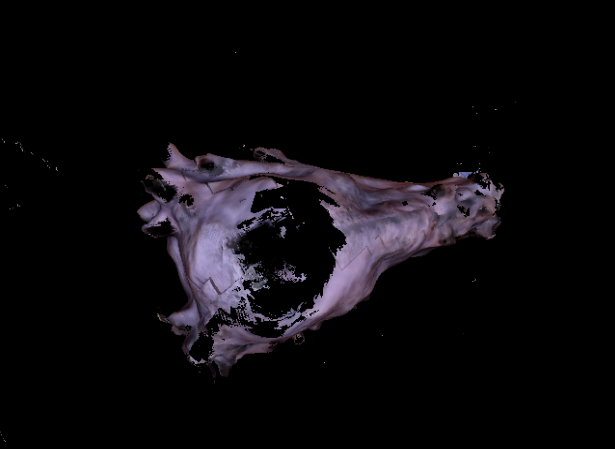
\includegraphics[width=2.5cm]{screenshots/dino_colour_top.PNG}}}&
		\bmvaHangBox{\fbox{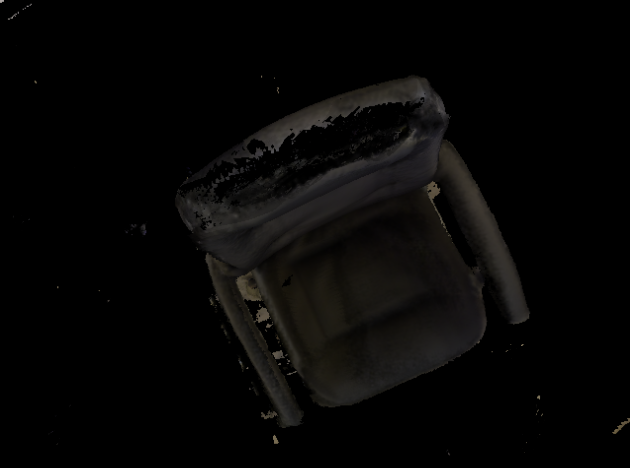
\includegraphics[width=2.5cm]{screenshots/chair_colour_top.PNG}}}&
		\bmvaHangBox{\fbox{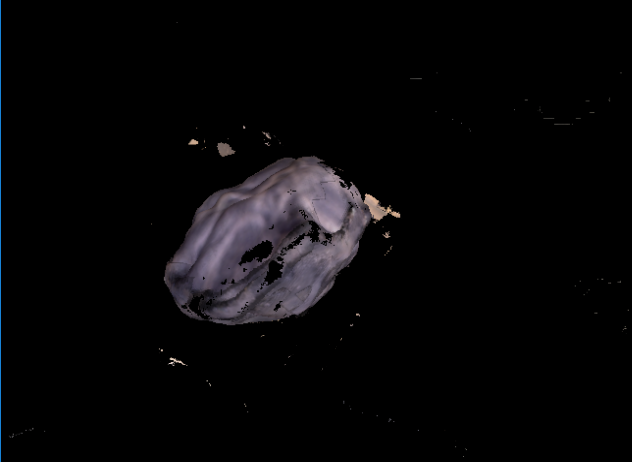
\includegraphics[width=2.5cm]{screenshots/rock_colour_top.PNG}}}\\
		(a)&(b)&(c)
	\end{tabular}
	\caption{
		\textbf{(a)} Closed reconstruction of a Dinosaur Head.
		\textbf{(b)} Closed reconstruction of a Chair.
		\textbf{(c)} Closed reconstruction of a Rock.
	}
	\label{fig:top_shots}
\end{figure}

As can be seen from the top down views of Figure \ref{fig:top_shots}, our system is capable of producing closed models, unaffected by tracking drift and loop closure events.